% Created by tikzDevice version 0.12.6 on 2024-06-11 19:57:13
% !TEX encoding = UTF-8 Unicode
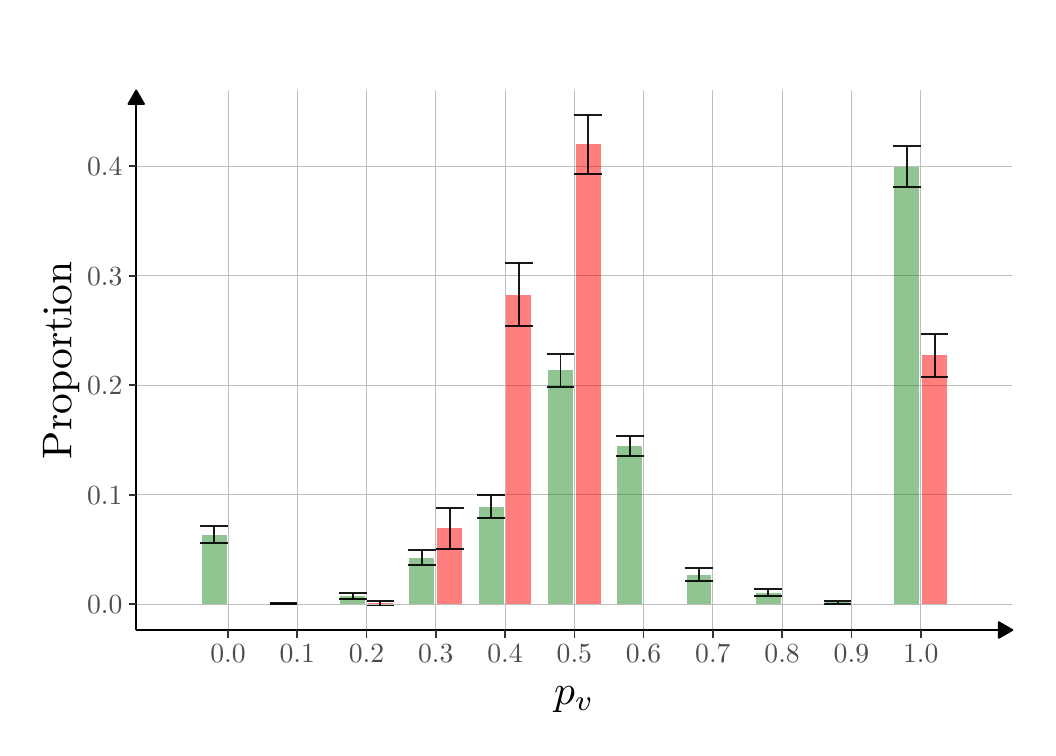
\begin{tikzpicture}[x=1pt,y=1pt]
\definecolor{fillColor}{RGB}{255,255,255}
\path[use as bounding box,fill=fillColor,fill opacity=0.00] (0,0) rectangle (361.35,252.94);
\begin{scope}
\path[clip] (  0.00,  0.00) rectangle (361.35,252.94);
\definecolor{drawColor}{RGB}{255,255,255}
\definecolor{fillColor}{RGB}{255,255,255}

\path[draw=drawColor,line width= 0.6pt,line join=round,line cap=round,fill=fillColor] (  0.00,  0.00) rectangle (361.35,252.94);
\end{scope}
\begin{scope}
\path[clip] ( 39.22, 35.28) rectangle (355.85,230.29);
\definecolor{fillColor}{RGB}{255,255,255}

\path[fill=fillColor] ( 39.22, 35.28) rectangle (355.85,230.29);
\definecolor{drawColor}{RGB}{255,255,255}

\path[draw=drawColor,line width= 0.3pt,line join=round] ( 39.22, 64.38) --
	(355.85, 64.38);

\path[draw=drawColor,line width= 0.3pt,line join=round] ( 39.22,103.94) --
	(355.85,103.94);

\path[draw=drawColor,line width= 0.3pt,line join=round] ( 39.22,143.51) --
	(355.85,143.51);

\path[draw=drawColor,line width= 0.3pt,line join=round] ( 39.22,183.08) --
	(355.85,183.08);

\path[draw=drawColor,line width= 0.3pt,line join=round] ( 39.22,222.65) --
	(355.85,222.65);

\path[draw=drawColor,line width= 0.3pt,line join=round] ( 47.36, 35.28) --
	( 47.36,230.29);

\path[draw=drawColor,line width= 0.3pt,line join=round] ( 59.87, 35.28) --
	( 59.87,230.29);

\path[draw=drawColor,line width= 0.3pt,line join=round] ( 84.90, 35.28) --
	( 84.90,230.29);

\path[draw=drawColor,line width= 0.3pt,line join=round] (109.93, 35.28) --
	(109.93,230.29);

\path[draw=drawColor,line width= 0.3pt,line join=round] (134.96, 35.28) --
	(134.96,230.29);

\path[draw=drawColor,line width= 0.3pt,line join=round] (159.99, 35.28) --
	(159.99,230.29);

\path[draw=drawColor,line width= 0.3pt,line join=round] (185.02, 35.28) --
	(185.02,230.29);

\path[draw=drawColor,line width= 0.3pt,line join=round] (210.05, 35.28) --
	(210.05,230.29);

\path[draw=drawColor,line width= 0.3pt,line join=round] (235.08, 35.28) --
	(235.08,230.29);

\path[draw=drawColor,line width= 0.3pt,line join=round] (260.11, 35.28) --
	(260.11,230.29);

\path[draw=drawColor,line width= 0.3pt,line join=round] (285.14, 35.28) --
	(285.14,230.29);

\path[draw=drawColor,line width= 0.3pt,line join=round] (310.17, 35.28) --
	(310.17,230.29);

\path[draw=drawColor,line width= 0.3pt,line join=round] (335.20, 35.28) --
	(335.20,230.29);

\path[draw=drawColor,line width= 0.3pt,line join=round] (347.72, 35.28) --
	(347.72,230.29);
\definecolor{drawColor}{RGB}{190,190,190}

\path[draw=drawColor,line width= 0.3pt,line join=round] ( 39.22, 44.59) --
	(355.85, 44.59);

\path[draw=drawColor,line width= 0.3pt,line join=round] ( 39.22, 84.16) --
	(355.85, 84.16);

\path[draw=drawColor,line width= 0.3pt,line join=round] ( 39.22,123.73) --
	(355.85,123.73);

\path[draw=drawColor,line width= 0.3pt,line join=round] ( 39.22,163.30) --
	(355.85,163.30);

\path[draw=drawColor,line width= 0.3pt,line join=round] ( 39.22,202.86) --
	(355.85,202.86);

\path[draw=drawColor,line width= 0.3pt,line join=round] ( 72.39, 35.28) --
	( 72.39,230.29);

\path[draw=drawColor,line width= 0.3pt,line join=round] ( 97.42, 35.28) --
	( 97.42,230.29);

\path[draw=drawColor,line width= 0.3pt,line join=round] (122.45, 35.28) --
	(122.45,230.29);

\path[draw=drawColor,line width= 0.3pt,line join=round] (147.48, 35.28) --
	(147.48,230.29);

\path[draw=drawColor,line width= 0.3pt,line join=round] (172.51, 35.28) --
	(172.51,230.29);

\path[draw=drawColor,line width= 0.3pt,line join=round] (197.54, 35.28) --
	(197.54,230.29);

\path[draw=drawColor,line width= 0.3pt,line join=round] (222.57, 35.28) --
	(222.57,230.29);

\path[draw=drawColor,line width= 0.3pt,line join=round] (247.60, 35.28) --
	(247.60,230.29);

\path[draw=drawColor,line width= 0.3pt,line join=round] (272.63, 35.28) --
	(272.63,230.29);

\path[draw=drawColor,line width= 0.3pt,line join=round] (297.66, 35.28) --
	(297.66,230.29);

\path[draw=drawColor,line width= 0.3pt,line join=round] (322.69, 35.28) --
	(322.69,230.29);
\definecolor{fillColor}{RGB}{34,139,34}

\path[fill=fillColor,fill opacity=0.50] ( 62.87, 44.59) rectangle ( 71.89, 69.72);

\path[fill=fillColor,fill opacity=0.50] ( 87.90, 44.59) rectangle ( 96.92, 44.82);

\path[fill=fillColor,fill opacity=0.50] (112.93, 44.59) rectangle (121.95, 47.49);

\path[fill=fillColor,fill opacity=0.50] (137.96, 44.59) rectangle (146.98, 61.44);

\path[fill=fillColor,fill opacity=0.50] (162.99, 44.59) rectangle (172.01, 79.78);

\path[fill=fillColor,fill opacity=0.50] (188.02, 44.59) rectangle (197.04,129.10);

\path[fill=fillColor,fill opacity=0.50] (213.05, 44.59) rectangle (222.07,101.74);

\path[fill=fillColor,fill opacity=0.50] (238.08, 44.59) rectangle (247.09, 55.23);

\path[fill=fillColor,fill opacity=0.50] (263.11, 44.59) rectangle (272.12, 48.79);

\path[fill=fillColor,fill opacity=0.50] (288.14, 44.59) rectangle (297.15, 45.31);

\path[fill=fillColor,fill opacity=0.50] (313.17, 44.59) rectangle (322.18,202.77);
\definecolor{fillColor}{RGB}{255,0,0}

\path[fill=fillColor,fill opacity=0.50] (122.95, 44.59) rectangle (131.96, 44.96);

\path[fill=fillColor,fill opacity=0.50] (147.98, 44.59) rectangle (156.99, 72.00);

\path[fill=fillColor,fill opacity=0.50] (173.01, 44.59) rectangle (182.02,156.45);

\path[fill=fillColor,fill opacity=0.50] (198.04, 44.59) rectangle (207.05,210.75);

\path[fill=fillColor,fill opacity=0.50] (323.19, 44.59) rectangle (332.20,134.48);
\definecolor{drawColor}{RGB}{0,0,0}

\path[draw=drawColor,draw opacity=0.90,line width= 0.7pt,line join=round] ( 62.37, 72.86) --
	( 72.39, 72.86);

\path[draw=drawColor,draw opacity=0.90,line width= 0.7pt,line join=round] ( 67.38, 72.86) --
	( 67.38, 66.58);

\path[draw=drawColor,draw opacity=0.90,line width= 0.7pt,line join=round] ( 62.37, 66.58) --
	( 72.39, 66.58);

\path[draw=drawColor,draw opacity=0.90,line width= 0.7pt,line join=round] ( 87.40, 45.13) --
	( 97.42, 45.13);

\path[draw=drawColor,draw opacity=0.90,line width= 0.7pt,line join=round] ( 92.41, 45.13) --
	( 92.41, 44.52);

\path[draw=drawColor,draw opacity=0.90,line width= 0.7pt,line join=round] ( 87.40, 44.52) --
	( 97.42, 44.52);

\path[draw=drawColor,draw opacity=0.90,line width= 0.7pt,line join=round] (112.43, 48.59) --
	(122.45, 48.59);

\path[draw=drawColor,draw opacity=0.90,line width= 0.7pt,line join=round] (117.44, 48.59) --
	(117.44, 46.39);

\path[draw=drawColor,draw opacity=0.90,line width= 0.7pt,line join=round] (112.43, 46.39) --
	(122.45, 46.39);

\path[draw=drawColor,draw opacity=0.90,line width= 0.7pt,line join=round] (137.46, 64.11) --
	(147.48, 64.11);

\path[draw=drawColor,draw opacity=0.90,line width= 0.7pt,line join=round] (142.47, 64.11) --
	(142.47, 58.78);

\path[draw=drawColor,draw opacity=0.90,line width= 0.7pt,line join=round] (137.46, 58.78) --
	(147.48, 58.78);

\path[draw=drawColor,draw opacity=0.90,line width= 0.7pt,line join=round] (162.49, 83.92) --
	(172.51, 83.92);

\path[draw=drawColor,draw opacity=0.90,line width= 0.7pt,line join=round] (167.50, 83.92) --
	(167.50, 75.64);

\path[draw=drawColor,draw opacity=0.90,line width= 0.7pt,line join=round] (162.49, 75.64) --
	(172.51, 75.64);

\path[draw=drawColor,draw opacity=0.90,line width= 0.7pt,line join=round] (187.52,134.98) --
	(197.54,134.98);

\path[draw=drawColor,draw opacity=0.90,line width= 0.7pt,line join=round] (192.53,134.98) --
	(192.53,123.22);

\path[draw=drawColor,draw opacity=0.90,line width= 0.7pt,line join=round] (187.52,123.22) --
	(197.54,123.22);

\path[draw=drawColor,draw opacity=0.90,line width= 0.7pt,line join=round] (212.55,105.32) --
	(222.57,105.32);

\path[draw=drawColor,draw opacity=0.90,line width= 0.7pt,line join=round] (217.56,105.32) --
	(217.56, 98.16);

\path[draw=drawColor,draw opacity=0.90,line width= 0.7pt,line join=round] (212.55, 98.16) --
	(222.57, 98.16);

\path[draw=drawColor,draw opacity=0.90,line width= 0.7pt,line join=round] (237.58, 57.55) --
	(247.60, 57.55);

\path[draw=drawColor,draw opacity=0.90,line width= 0.7pt,line join=round] (242.59, 57.55) --
	(242.59, 52.90);

\path[draw=drawColor,draw opacity=0.90,line width= 0.7pt,line join=round] (237.58, 52.90) --
	(247.60, 52.90);

\path[draw=drawColor,draw opacity=0.90,line width= 0.7pt,line join=round] (262.61, 50.11) --
	(272.63, 50.11);

\path[draw=drawColor,draw opacity=0.90,line width= 0.7pt,line join=round] (267.62, 50.11) --
	(267.62, 47.48);

\path[draw=drawColor,draw opacity=0.90,line width= 0.7pt,line join=round] (262.61, 47.48) --
	(272.63, 47.48);

\path[draw=drawColor,draw opacity=0.90,line width= 0.7pt,line join=round] (287.64, 45.85) --
	(297.66, 45.85);

\path[draw=drawColor,draw opacity=0.90,line width= 0.7pt,line join=round] (292.65, 45.85) --
	(292.65, 44.78);

\path[draw=drawColor,draw opacity=0.90,line width= 0.7pt,line join=round] (287.64, 44.78) --
	(297.66, 44.78);

\path[draw=drawColor,draw opacity=0.90,line width= 0.7pt,line join=round] (312.67,210.14) --
	(322.69,210.14);

\path[draw=drawColor,draw opacity=0.90,line width= 0.7pt,line join=round] (317.68,210.14) --
	(317.68,195.39);

\path[draw=drawColor,draw opacity=0.90,line width= 0.7pt,line join=round] (312.67,195.39) --
	(322.69,195.39);

\path[draw=drawColor,draw opacity=0.90,line width= 0.7pt,line join=round] (122.45, 45.78) --
	(132.46, 45.78);

\path[draw=drawColor,draw opacity=0.90,line width= 0.7pt,line join=round] (127.45, 45.78) --
	(127.45, 44.14);

\path[draw=drawColor,draw opacity=0.90,line width= 0.7pt,line join=round] (122.45, 44.14) --
	(132.46, 44.14);

\path[draw=drawColor,draw opacity=0.90,line width= 0.7pt,line join=round] (147.48, 79.30) --
	(157.49, 79.30);

\path[draw=drawColor,draw opacity=0.90,line width= 0.7pt,line join=round] (152.48, 79.30) --
	(152.48, 64.69);

\path[draw=drawColor,draw opacity=0.90,line width= 0.7pt,line join=round] (147.48, 64.69) --
	(157.49, 64.69);

\path[draw=drawColor,draw opacity=0.90,line width= 0.7pt,line join=round] (172.51,167.80) --
	(182.52,167.80);

\path[draw=drawColor,draw opacity=0.90,line width= 0.7pt,line join=round] (177.51,167.80) --
	(177.51,145.11);

\path[draw=drawColor,draw opacity=0.90,line width= 0.7pt,line join=round] (172.51,145.11) --
	(182.52,145.11);

\path[draw=drawColor,draw opacity=0.90,line width= 0.7pt,line join=round] (197.54,221.42) --
	(207.55,221.42);

\path[draw=drawColor,draw opacity=0.90,line width= 0.7pt,line join=round] (202.54,221.42) --
	(202.54,200.07);

\path[draw=drawColor,draw opacity=0.90,line width= 0.7pt,line join=round] (197.54,200.07) --
	(207.55,200.07);

\path[draw=drawColor,draw opacity=0.90,line width= 0.7pt,line join=round] (322.69,142.11) --
	(332.70,142.11);

\path[draw=drawColor,draw opacity=0.90,line width= 0.7pt,line join=round] (327.69,142.11) --
	(327.69,126.86);

\path[draw=drawColor,draw opacity=0.90,line width= 0.7pt,line join=round] (322.69,126.86) --
	(332.70,126.86);
\end{scope}
\begin{scope}
\path[clip] (  0.00,  0.00) rectangle (361.35,252.94);
\definecolor{drawColor}{RGB}{0,0,0}

\path[draw=drawColor,line width= 0.6pt,line join=round] ( 39.22, 35.28) --
	( 39.22,230.29);
\definecolor{fillColor}{RGB}{0,0,0}

\path[draw=drawColor,line width= 0.6pt,line join=round,fill=fillColor] ( 42.07,225.36) --
	( 39.22,230.29) --
	( 36.38,225.36) --
	cycle;
\end{scope}
\begin{scope}
\path[clip] (  0.00,  0.00) rectangle (361.35,252.94);
\definecolor{drawColor}{gray}{0.30}

\node[text=drawColor,anchor=base east,inner sep=0pt, outer sep=0pt, scale=  1.00] at ( 34.27, 41.15) {0.0};

\node[text=drawColor,anchor=base east,inner sep=0pt, outer sep=0pt, scale=  1.00] at ( 34.27, 80.72) {0.1};

\node[text=drawColor,anchor=base east,inner sep=0pt, outer sep=0pt, scale=  1.00] at ( 34.27,120.28) {0.2};

\node[text=drawColor,anchor=base east,inner sep=0pt, outer sep=0pt, scale=  1.00] at ( 34.27,159.85) {0.3};

\node[text=drawColor,anchor=base east,inner sep=0pt, outer sep=0pt, scale=  1.00] at ( 34.27,199.42) {0.4};
\end{scope}
\begin{scope}
\path[clip] (  0.00,  0.00) rectangle (361.35,252.94);
\definecolor{drawColor}{gray}{0.20}

\path[draw=drawColor,line width= 0.6pt,line join=round] ( 36.47, 44.59) --
	( 39.22, 44.59);

\path[draw=drawColor,line width= 0.6pt,line join=round] ( 36.47, 84.16) --
	( 39.22, 84.16);

\path[draw=drawColor,line width= 0.6pt,line join=round] ( 36.47,123.73) --
	( 39.22,123.73);

\path[draw=drawColor,line width= 0.6pt,line join=round] ( 36.47,163.30) --
	( 39.22,163.30);

\path[draw=drawColor,line width= 0.6pt,line join=round] ( 36.47,202.86) --
	( 39.22,202.86);
\end{scope}
\begin{scope}
\path[clip] (  0.00,  0.00) rectangle (361.35,252.94);
\definecolor{drawColor}{RGB}{0,0,0}

\path[draw=drawColor,line width= 0.6pt,line join=round] ( 39.22, 35.28) --
	(355.85, 35.28);
\definecolor{fillColor}{RGB}{0,0,0}

\path[draw=drawColor,line width= 0.6pt,line join=round,fill=fillColor] (350.92, 32.43) --
	(355.85, 35.28) --
	(350.92, 38.12) --
	cycle;
\end{scope}
\begin{scope}
\path[clip] (  0.00,  0.00) rectangle (361.35,252.94);
\definecolor{drawColor}{gray}{0.20}

\path[draw=drawColor,line width= 0.6pt,line join=round] ( 72.39, 32.53) --
	( 72.39, 35.28);

\path[draw=drawColor,line width= 0.6pt,line join=round] ( 97.42, 32.53) --
	( 97.42, 35.28);

\path[draw=drawColor,line width= 0.6pt,line join=round] (122.45, 32.53) --
	(122.45, 35.28);

\path[draw=drawColor,line width= 0.6pt,line join=round] (147.48, 32.53) --
	(147.48, 35.28);

\path[draw=drawColor,line width= 0.6pt,line join=round] (172.51, 32.53) --
	(172.51, 35.28);

\path[draw=drawColor,line width= 0.6pt,line join=round] (197.54, 32.53) --
	(197.54, 35.28);

\path[draw=drawColor,line width= 0.6pt,line join=round] (222.57, 32.53) --
	(222.57, 35.28);

\path[draw=drawColor,line width= 0.6pt,line join=round] (247.60, 32.53) --
	(247.60, 35.28);

\path[draw=drawColor,line width= 0.6pt,line join=round] (272.63, 32.53) --
	(272.63, 35.28);

\path[draw=drawColor,line width= 0.6pt,line join=round] (297.66, 32.53) --
	(297.66, 35.28);

\path[draw=drawColor,line width= 0.6pt,line join=round] (322.69, 32.53) --
	(322.69, 35.28);
\end{scope}
\begin{scope}
\path[clip] (  0.00,  0.00) rectangle (361.35,252.94);
\definecolor{drawColor}{gray}{0.30}

\node[text=drawColor,anchor=base,inner sep=0pt, outer sep=0pt, scale=  1.00] at ( 72.39, 23.44) {0.0};

\node[text=drawColor,anchor=base,inner sep=0pt, outer sep=0pt, scale=  1.00] at ( 97.42, 23.44) {0.1};

\node[text=drawColor,anchor=base,inner sep=0pt, outer sep=0pt, scale=  1.00] at (122.45, 23.44) {0.2};

\node[text=drawColor,anchor=base,inner sep=0pt, outer sep=0pt, scale=  1.00] at (147.48, 23.44) {0.3};

\node[text=drawColor,anchor=base,inner sep=0pt, outer sep=0pt, scale=  1.00] at (172.51, 23.44) {0.4};

\node[text=drawColor,anchor=base,inner sep=0pt, outer sep=0pt, scale=  1.00] at (197.54, 23.44) {0.5};

\node[text=drawColor,anchor=base,inner sep=0pt, outer sep=0pt, scale=  1.00] at (222.57, 23.44) {0.6};

\node[text=drawColor,anchor=base,inner sep=0pt, outer sep=0pt, scale=  1.00] at (247.60, 23.44) {0.7};

\node[text=drawColor,anchor=base,inner sep=0pt, outer sep=0pt, scale=  1.00] at (272.63, 23.44) {0.8};

\node[text=drawColor,anchor=base,inner sep=0pt, outer sep=0pt, scale=  1.00] at (297.66, 23.44) {0.9};

\node[text=drawColor,anchor=base,inner sep=0pt, outer sep=0pt, scale=  1.00] at (322.69, 23.44) {1.0};
\end{scope}
\begin{scope}
\path[clip] (  0.00,  0.00) rectangle (361.35,252.94);
\definecolor{drawColor}{RGB}{0,0,0}

\node[text=drawColor,anchor=base,inner sep=0pt, outer sep=0pt, scale=  1.50] at (197.54,  8.42) {$p_v$};
\end{scope}
\begin{scope}
\path[clip] (  0.00,  0.00) rectangle (361.35,252.94);
\definecolor{drawColor}{RGB}{0,0,0}

\node[text=drawColor,rotate= 90.00,anchor=base,inner sep=0pt, outer sep=0pt, scale=  1.50] at ( 15.83,132.78) {Proportion};
\end{scope}
\end{tikzpicture}
